%----------------------------------------------------------------------------------------
%    PACKAGES AND OTHER DOCUMENT CONFIGURATIONS
%----------------------------------------------------------------------------------------

\documentclass[paper=a4, fontsize=11pt]{scrartcl} % A4 paper and 11pt font size

%----------------------------------------------------------------------------------------
%    CODIFICACIÓ TEXT I IDIOMA
%----------------------------------------------------------------------------------------
%%\usepackage[utf8]{inputenc}
\usepackage[scaled]{beramono}
%\renewcommand*\ttdefault{cmr}
%\renewcommand*\familydefault{\ttdefault} %% Only if the base font of the document is to be typewriter style

\usepackage[T1]{fontenc}
%\usepackage{fontenc}
%\usepackage{classicthesis}
%\usepackage[catalan]{babel}  % Utilitzar idioma català amb accents
\usepackage[english]{babel}
\usepackage{mathpazo}

%\usepackage{fourier} % Use the Adobe Utopia font for the document - comment this line to return to the LaTeX default

%----------------------------------------------------------------------------------------
%    PAQUETS MATEMÀTICS I IMATGES
%----------------------------------------------------------------------------------------
\usepackage{amsmath,amsfonts,amsthm} % Math packages
\DeclareMathOperator{\sgn}{sgn}
\newcommand\abs[1]{\left|#1\right|}
\usepackage{tikz}
\usepackage{pgfplots}
\usepackage{graphicx}
\usepackage[framed,numbered,autolinebreaks,useliterate]{mcode}
\lstset{breakatwhitespace=false}
\lstset{captionpos=b}
\usepackage{booktabs}
\usepackage{hyperref}
\usepackage{color}
\usepackage{natbib}
\newtheorem{theorem}{Theorem}[subsection]
\newtheorem{statement}[theorem]{Statement}
\newtheorem{definition}[theorem]{definition}
\renewcommand{\lstlistingname}{Code}% Listing -> Code
\usepackage{float}

%----------------------------------------------------------------------------------------
%    PAGINACIÓ I COSES PER QUE QUEDI MÉS MACO
%----------------------------------------------------------------------------------------
\usepackage{sectsty} % Allows customizing section commands
\allsectionsfont{\normalfont\bf\renewcommand{\baselinestretch}{2}} % Lletra normal i negreta

\usepackage{lastpage} % Required to determine the last page for the footer
\usepackage{extramarks} % Required for headers and footers
\usepackage{fancyhdr} % Custom headers and footers
\pagestyle{fancy} % Makes all pages in the document conform to the custom headers and footers
\fancyhead{} % No page header - if you want one, create it in the same way as the footers below
\fancyfoot[L]{} % Empty left footer
\fancyfoot[C]{} % Empty center footer
\fancyfoot[R]{\thepage} % Page numbering for right footer
\renewcommand{\headrulewidth}{0pt} % Remove header underlines
\renewcommand{\footrulewidth}{0pt} % Remove footer underlines
\setlength{\headheight}{13.6pt} % Customize the height of the header
\textheight = 650pt
\usepackage[labelfont=bf]{caption} %Serveix per a que les llegendes de les taules siguin amb negreta la part Taula 1, Taula 2 ec...
\newcommand{\horrule}[1]{\rule{\linewidth}{#1}}

\usepackage{euler}
%\usepackage[nochapters]{classicthesis}

%\numberwithin{equation}{section} % Number equations within sections (i.e. 1.1, 1.2, 2.1, 2.2 instead of 1, 2, 3, 4)
%\numberwithin{figure}{section} % Number figures within sections (i.e. 1.1, 1.2, 2.1, 2.2 instead of 1, 2, 3, 4)
%\numberwithin{table}{section} % Number tables within sections (i.e. 1.1, 1.2, 2.1, 2.2 instead of 1, 2, 3, 4)

\setlength\parindent{0pt}

% \title{Mini Project 1: \\Position Analysis of wing mechanisms and quadrotor formations}

% \author{Ferran Plana Rius \\ Jordi Soler Busquets}

\title{	\pagestyle{empty}
\normalfont \normalsize 
\textsc{Polytechnic University of Catalonia} \\ [25pt] % Your university, school and/or  department name(s)
\horrule{0.5pt} \\[0.4cm] % Thin top horizontal rule 
\Huge \bf Mini Project 1 \\ % The assignment title
\large Position Analysis of wing mechanisms and quadrotor formations
\horrule{2pt} \\[0.5cm] % Thick bottom horizontal rule
\textsc{Geometric Fundamentals for Robot Design} \\ [25pt]
}

%----------------------------------------------------------------------------------------
%    AUTORS
%----------------------------------------------------------------------------------------
\author{\bf{Ferran Plana Rius}\\ \small{Master's AiR student, UPC} \\ \small{nandoplana@gmail.com} \\ \\
\bf{Jordi Soler Busquets}\\ \small{Master's AiR student, UPC} \\ \small{jordi.solerbusquets@gmail.com} \\ \\}
\date{\large\today}

%\date{\today}
\begin{document}
% \renewcommand{\headheight}{0.6in}
% \setlength{\headwidth}{\textwidth}
% \fancyhead[L]{
\includegraphics[height=0.35in]{UPC-logo.png}% empty left
% \fancyhead[R]{Geometric Fundamentals\\ for Robotic Design\\ \tiny Master's degree in\\ Automatic Control and Robotics} % right  
%  }
% \pagestyle{fancyplain}
% \maketitle

\pagestyle{empty}
\maketitle % Print the title
\begin{figure}[b]
  \centering
     
\includegraphics[width=0.7\textwidth]{UPC-logo.png}
\end{figure}
\thispagestyle{empty}
\newpage
\pagestyle{fancyplain}
\renewcommand\footrulewidth{0.1pt} % Size of the footer rule
\rfoot{Page \thepage\ of\ \pageref{LastPage}}


In the mini project presented here, we are asked to put in practice all we have learned during the course, regarding the position analysis methods. As a first exercise it will be simulated the Smartbird's wing mechanism, which is constructible and can be analyzed using the Geaogebra software. The second exercise consists in the position analysis of a quadrotor localization problem, an equivalent 3-R\underline{P}R structure, which is no constructible, hence CUIK is a useful tool in this case.

\section{Simulation of Smartbird's wing}
Figure \ref{fig:wing} shows the mechanical structure of Smartbird's wing. Every small circle represents a revolute joint and vertexs A and B are attached to the body (ground).\\
	
\begin{figure}[htb]
	\begin{center}
		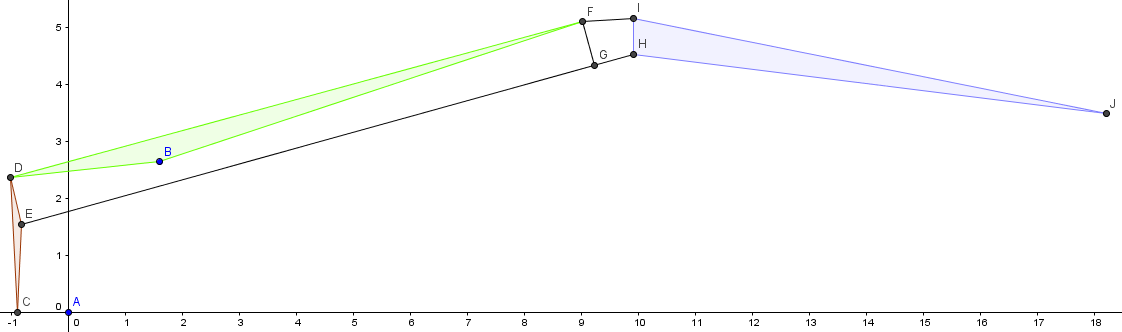
\includegraphics[width=0.75\linewidth]{wing.PNG} 
	\caption{Mechanical structure of Smartbird's wing}
	\label{fig:wing}
	\end{center}
\end{figure}

\subsection*{First Step}
To start with, it will be proved that the mechanism of the Figure \ref{fig:wing} is constructive, describing its connections and bilaterations operations.
\begin{enumerate}
\item Known points $A$ and $B$ are set to their locations: $A=(0,0)$ and $B=(1.596,2.638)$
\item An angle $\theta$ is created in order to place the point $C$ with respect to the horizontal line. With that angle and the distance $\overline{AC}$ the point $C$ is placed.
\item Knowing the distances $\overline{CD}$ and $\overline{BD}$ point $B$ and $C$ are bilaterated to find $D$
\item Bilateratinf $C$ and $D$ with the proper distances, the point $E$ is placed.
\item With the same procedure, points $B$ and $D$ and $\overline{BF}$ and $\overline{DF}$ point $F$ is placed.
\item Drawing a circle over $F$ with disctance $\overline{FG}$ and finding the one of its tangents passing through $E$, point $G$ is found as the tangent point.
\item Computing the intersction between the previous tangent and a circle centered in $E$ with radious $\overline{EH}$ point $H$ is placed.
\item Bilaterating $F$ and $H$ with the proper lengths, $I$ is placed.
\item Bilaterating $H$ and $I$ with the proper lengths, $J$ is placed.
\end{enumerate}

\subsection*{Second Step}
Next, it is built the smartbird's wing mechanism in the Geogebra software. At the end, it is obtained the resultant structure shown in the Figure \ref{fig:wing}. A \emph{ggb} file showing the result is attached.

\subsection*{Third Step}
As the exercise ask, it is activated the motion of the link AC by using the angle variable $\theta$. Next, it is added the trace of the vertex F, H and J. The results of this operation can be seen in the Figure \ref{fig:wing_result}.
\begin{figure}[htb]
	\begin{center}
		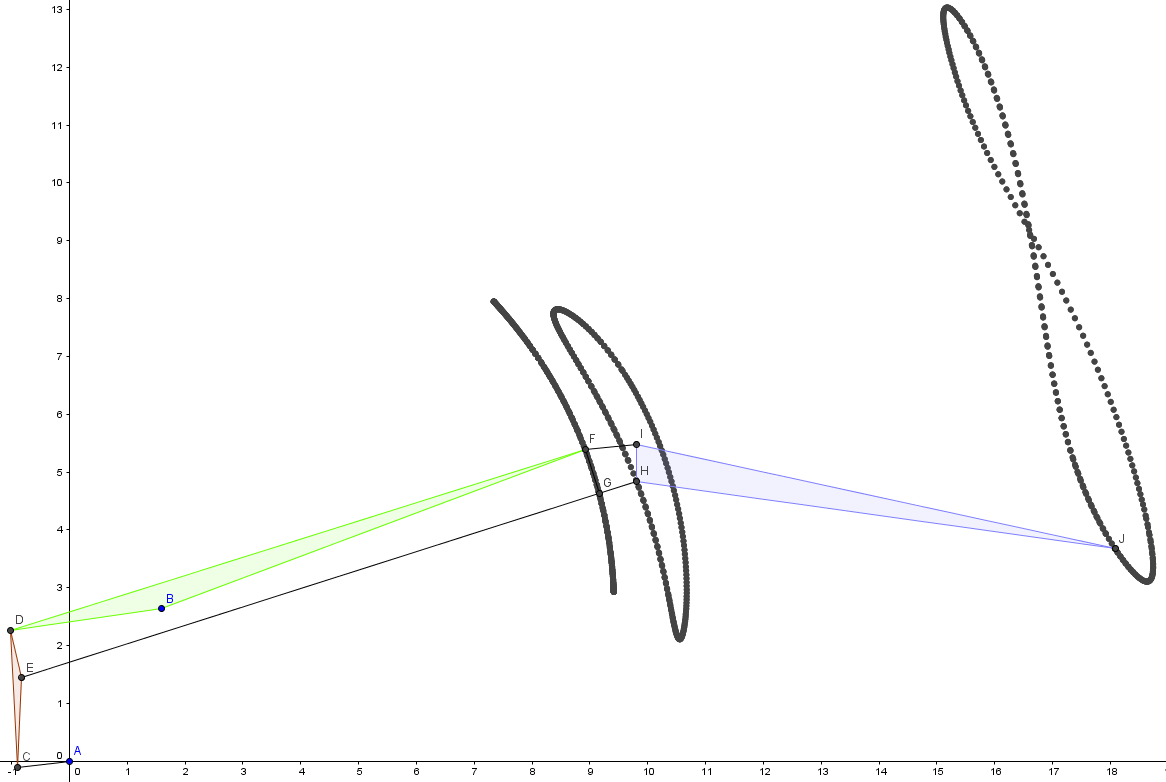
\includegraphics[width=0.5\linewidth]{wing_result.png} 
	\caption{Trace of vertex F, H and J}
	\label{fig:wing_result}
	\end{center}
\end{figure}

\section{Quadrotor localization}
\subsection*{Problem formulation}
The problem  can be formulated by using distance constraints of the form $(x_i-x_j)^2+(y_i-y_j)^2 = d_{ij}^2$.  This constraints should be applied to all the measured and known distances. We need to take into account the angle $\theta$. Furthermore, we know that point 1 is located at the origin and the position of sensor 2 is in the $x$ axis.
\begin{figure}[H]
	\begin{center}
		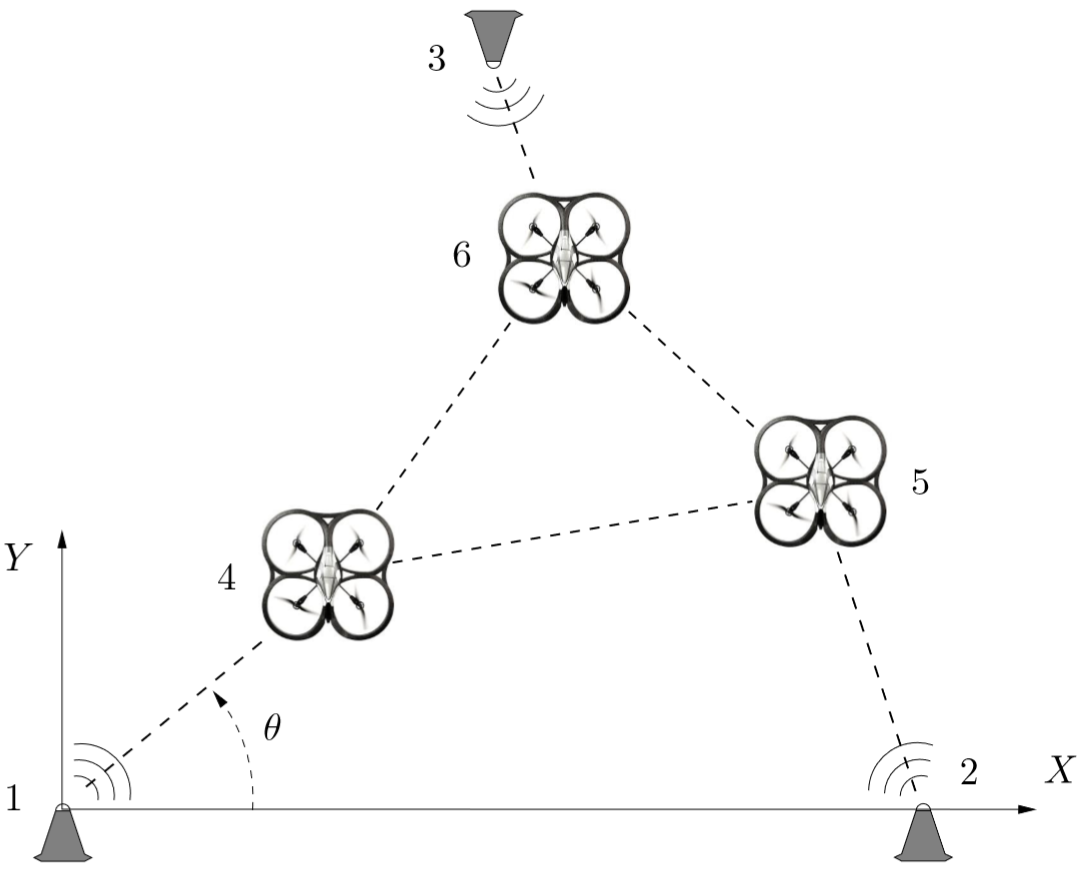
\includegraphics[width=0.4\linewidth]{quad.PNG} 
	\caption{Problem description}
	\label{fig:quad}
	\end{center}
\end{figure}

Given the previous information we have:

\begin{align}
& x_1 = 0\\
& y_1 = 0\\
& y_2 = 0\\
& x_4 = cos(\theta)d_{14}\\
& y_4 = sin(\theta)d_{14}\\
& (x_1-x_2)^2+(y_1-y_2)^2 = d_{12}^2\\
& (x_1-x_3)^2+(y_1-y_3)^2 = d_{13}^2\\
& (x_3-x_2)^2+(y_3-y_2)^2 = d_{32}^2\\
& (x_4-x_5)^2+(y_4-y_5)^2 = d_{45}^2\\
& (x_4-x_6)^2+(y_4-y_6)^2 = d_{46}^2\\
& (x_6-x_5)^2+(y_6-y_5)^2 = d_{65}^2\\
& (x_2-x_5)^2+(y_2-y_5)^2 = d_{25}^2\\
& (x_3-x_6)^2+(y_3-y_6)^2 = d_{36}^2
\end{align}
%\newpage
As CuikSuite does not deal with sinusoidal functions we can replaced the equations related to point 4 coordinates by:
\begin{align}
& x_4 = c_1d_{14}\\
& y_4 = s_1d_{14}\\
& c_1^2+s_1^2=0
\end{align}

The points 1, 2, 3 are fixed and known, and so are their coordinates. Hence, equations 1, 2, 3, 6, 7 and 8 can be considered as the definition of the framework. We still consider the angle $\theta$ unknown due to its uncertainty (it's value, although bounded, is unknown). Thus, we can consider the system of equations defining the problem as follows:
\begin{align}
\label{syseq1}
& (x_4-x_5)^2+(y_4-y_5)^2 = d_{45}^2\\
& (x_4-x_6)^2+(y_4-y_6)^2 = d_{46}^2\\
& (x_6-x_5)^2+(y_6-y_5)^2 = d_{65}^2\\
& (x_2-x_5)^2+(y_2-y_5)^2 = d_{25}^2\\
& (x_3-x_6)^2+(y_3-y_6)^2 = d_{36}^2\\
& x_4 = c_1d_{14}\\
& y_4 = s_1d_{14}\\
& c_1^2+s_1^2=1
\label{syseq2}
\end{align}

Being $x_4,\ y_4,\ x_5,\ y_5,\ x_6,\ y_6,\ s_1$ and $c_1$ unknowns and $x_1,\ y_1,\ x_2,\ y_2,\ x_3$ and $y_3$ are constants.


\subsection*{Forcing angular constraint}
We need to ensure that $\theta \in [\theta_{min}, \theta_{max}]$. As the angle is not directly a variable of our system but its sinus and cosinus, we can constrain its cosinus because 
\begin{equation}
\label{constr1}
cos(\alpha) \in [cos(\beta), 1]
\end{equation}
is equivalent to
\begin{equation}
\label{constr2}
\alpha \in [-\beta, \beta]
\end{equation}
So, given a constraint in the form of \ref{constr2} we can transform it to the form \ref{constr1}. It should be noticed that this procedure is only valid when $\theta_{min}=-\theta_{max}$, but not in a general case when the angle range is not centered in 0.

\subsection*{Analysis of the system}
We consider the system in \ref{syseq1}-\ref{syseq2}, so we have 8 equations. The number of variables, as stated in first section is also 8.

\subsection*{Box bounding}
In order to reduce the computational cost of the CUIK software, the problem can be bounded by reducing the dimension of the initial search box. Observing the Figure \ref{fig:quad} it can be seen that several circles are limiting how farther the quadrotors formation can be. Namely, if it is considered the distances $d_{14}$ and $d_{45}$, the point 5 can be as further as a circle of radius $d_{14}+d_{45}$. Hence, extending this conclusion to all the sides, it can be described the following limits. The distances between quadrotors are considered equal ($d_q$).

\begin{align}
&-d_{14}<x_4<d_{14} \\
&-d_{14}<y_4<d_{14} \\
&-d_{14}-d_q<x_5<d_{14}+d_q \\
&-d_{14}-d_q<y_5<d_{14}+d_q \\
&-d_{14}-d_q<x_6<d_{14}+d_q \\
&-d_{14}-d_q<y_6<d_{14}+d_q
\end{align}

Furthermore, since the cosine and sinus of the angel $\phi$ are considered as variables, they have to be limited between -1 to 1, or to another number depending the specifications of the problem.

\begin{align}
&-1<cos(\phi)<1 \\
&-1<sin(\phi)<1 
\end{align}

\subsection*{CUIK solver}
Now that the problem is well defined, it can be translated to the scribes needed for CUIK. First of all, the problems specifies a $\sigma=0.05$ that will be introduced in the *.param file, where all the CUIK solver parameters are defined. Next, it is created a new file *.cuik, where all the equations and constraints will be paced (see annex to check the final file). The statement propose three different configurations (Table \ref{tab:cases}) to be tested and evaluated. In further sections are shown the results.

\begin{table}[ht]
\begin{center}
	\begin{tabular}{ c c c c c c c c  }
 			Situation & $d_s$ & $d_q$ & $d_{14}$ & $d_{25}$ & $d_{3,5}$ & $\theta_{min}$ & $\theta_{min}$ \\
 			A & 3 & 1 & 2 & 2 & 2 & -3º & 3º \\
 			B & 3 & 1 & 2 & 2 & 2 & 0º & 60º \\
            C & 3 & 3 & 4 & 4 & 4 & 0º & 360º \\
	\end{tabular}
    \caption{Studying Cases}
    \label{tab:cases}
\end{center}
\end{table}

\subsection*{Quadrotor configurations}
In this section, The different solutions for every case are shown in the Figures \ref{fig:SolA}, \ref{fig:SolB} and \ref{fig:SolC}.

\begin{figure}[H]
	\begin{center}
		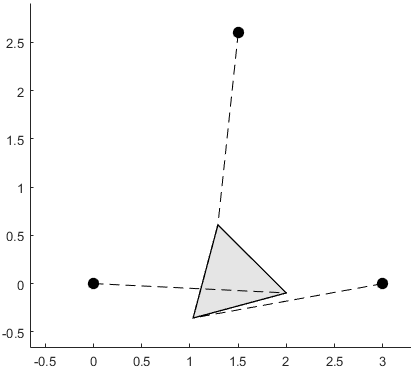
\includegraphics[width=0.5\linewidth]{SolA.png} 
	\caption{Unique solution of the system in case A}
	\label{fig:SolA}
	\end{center}
\end{figure}

For the first case, CUIK only give one solution (Figure \ref{fig:SolA}). This is produced due to the dimensions given to the different parameters, such as the distance between sensors ($d_s$), the distance between quadrotors ($d_q$) and the length imposed from quadrotor to sensor ($d_{14}$,$d_{36}$ and $d_{25}$).   

\begin{figure}[H]
	\begin{center}
		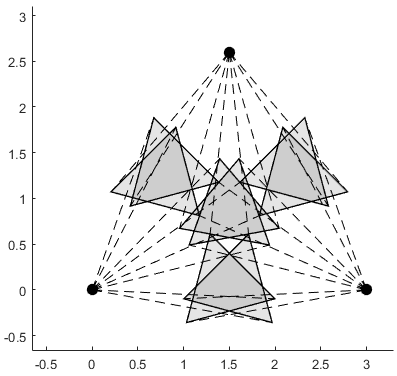
\includegraphics[width=0.5\linewidth]{SolB.png} 
	\caption{Solutions of the system in case B}
	\label{fig:SolB}
	\end{center}
\end{figure}

In the case B, the configuration between parameters allow the system adopt 8 solutions (Figure \ref{fig:SolB}). Hence, the solution is not unique.

\begin{figure}[H]
	\begin{center}
		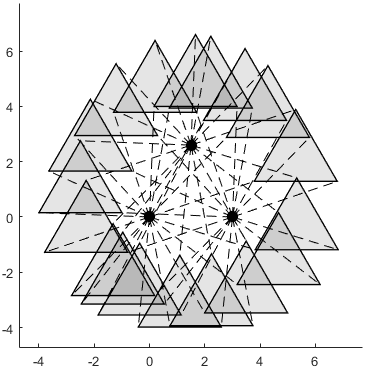
\includegraphics[width=0.6\linewidth]{SolC.png} 
	\caption{Some of the solutions of case C. Only some reduced number of solutions are plotted in order to obtain a clear image.}
	\label{fig:SolC}
	\end{center}
\end{figure}

The last configuration (case C) have considerable amount of solutions. In Figure \ref{fig:SolC} are draw several of them, however, a circle can be appreciated as the path followed by the possible configurations.

\subsection*{Observing variables $y_4$ and $x_5$}

\subsubsection*{Case A}
In this case, a single solution is found, so it is clear that there is only a single combination of $x_5$ and $y_4$ (a single point) that corresponds to a solution of the system.
\begin{figure}[H]
	\begin{center}
		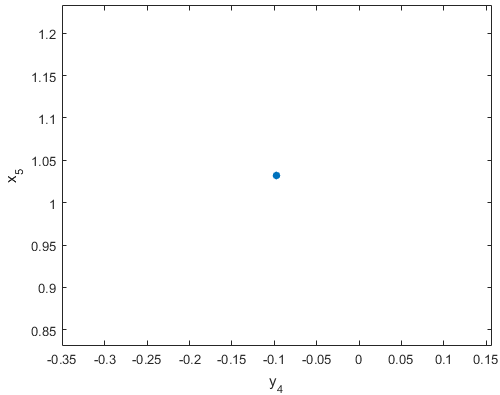
\includegraphics[width=0.44\linewidth]{p2D_A.png} 
	\caption{Variables $x_5$ and $y_4$ of the solutions of case A. Single point.}
	\label{fig:p2D_A}
	\end{center}
\end{figure}

\subsubsection*{Case B}
In this case, as the constraints are relaxed (allowing $\theta \in (0,\ 360)$) we observe many isolated points corresponding to a rotated/mirrored versions of the previous one. Still, we have a finite set of solution points.

\begin{figure}[H]
	\begin{center}
		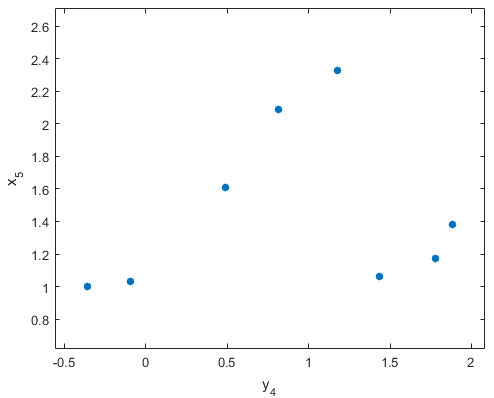
\includegraphics[width=0.55\linewidth]{p2D_B.png} 
	\caption{Variables $x_5$ and $y_4$ of the solutions of case B. Finite set of points.}
	\label{fig:p2D_B}
	\end{center}
\end{figure}

\subsubsection*{Case C}
Due to the particular geometry of this case (the triangle of sensors and quadrotors are the same and all sensor-quadrotor distances are also the same) the lines joining each quadrotor to its corresponding sensor are aligned. This gives rise to an infinite solution set. Intuitively as both quadrotor and sensor shapes are the same, regarding the closed curve, we can consider the system as composed by two points separated a certain distance. Thus, fixing one of them (for instance the sensor equivalent point) and moving the other we have a circular trajectory) as seen in figure \ref{fig:p2D_C}. 
\begin{figure}[H]
	\begin{center}
		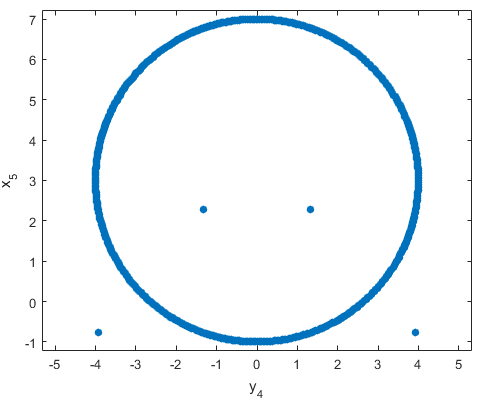
\includegraphics[width=0.5\linewidth]{p2D_C.png} 
	\caption{Variables $x_5$ and $y_4$ of the solutions of case C}
	\label{fig:p2D_C}
	\end{center}
\end{figure}

The isolated points correspond to configurations where sensor-quadrotor lines are not parallel and hence no movement can be done without changing the sensor-quadrotor distances. Figure \ref{7c} shows the four isolated points in figure \ref{fig:p2D_C}

\begin{figure}[H]
	\begin{center}
		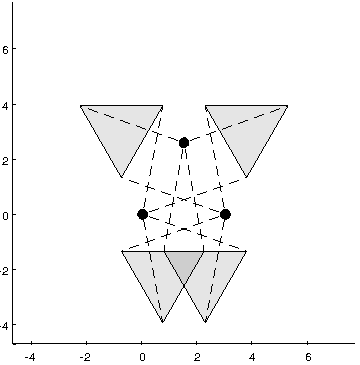
\includegraphics[width=0.5\linewidth]{7c.png} 
	\caption{Isolated configurations of case C}
	\label{7c}
	\end{center}
\end{figure}

\newpage
\section{Annex 1}
\begin{verbatim}
[CONSTANTS]

% Situation A
d14:=2.0
d25:=2.0
d36:=2.0
ds:=3.0
dq:=1.0
phimin:=-3.0*pi/180
phimax:=3.0*pi/180
X1:=0
Y1:=0
X2:=ds
Y2:=0
X3:=ds/2
Y3:=sin(pi/3)*ds

[SYSTEM VARS]

x4:[-d14,d14]
y4:[-d14,d14]
x5:[-d14-dq,d14+dq]
y5:[-d14-dq,d14+dq]
x6:[-d14-dq,d14+dq]
y6:[-d14-dq,d14+dq]
s1:[-1,1]
c1:[cos(phimin),1]
%c1:[-1,1]

[SYSTEM EQS]

% Distance equations
x4^2+x5^2-2*x5*x4+y4^2+y5^2-2*y5*y4 = dq^2;
X2^2+x5^2-2*x5*X2+Y2^2+y5^2-2*y5*Y2 = d25^2;
X3^2+x6^2-2*x6*X3+Y3^2+y6^2-2*y6*Y3 = d36^2;
x4^2+x6^2-2*x6*x4+y4^2+y6^2-2*y6*y4 = dq^2;
x6^2+x5^2-2*x5*x6+y6^2+y5^2-2*y5*y6 = dq^2;
x4 = d14*c1;
y4 = d14*s1;

% Circle equations
s1^2 + c1^2 = 1;
\end{verbatim}
\end{document}